\section{Projekt Narra}
\par Narra je projekt s volně dostupným zdrojovým kódem, který se zabývá anotací a~propojením audiovizuálních médií a~textu. Podobně jako YouTube má dostupné API a po dokončení bude soužit umělcům, filmařům a~dalším, kteří chtějí vytvářet otevřený příběh (Open Narrative), nebo editovat videa. Dokumentaristé mohou tento projekt využít pro rozsáhlejší díla, díky nabídnutému relevantnímu obsahu s metadaty. Projekt zastřešuje FAMU CAS a celý vývojářský tým tvoří 5 lidí, včetně studentů dokončujících Bakalářské a~Magisterské studium.
\par S první myšlenkou projektu Narra přišel v roce 2002 - 2003 Eric Rosenzveig a~Willy LeMaitre spolu s dalšími mediálními umělci a~programátory. Dílo bylo rozdělené na tři části. První\uv{playListNetWork} byl opensource software vyvinutý na základě konzultací s umělci o audiovizuálním obsahu a~rozhraním pro vizualizaci. Umožňoval práci více uživatelů na různých místech a~pomocí textových poznámek upravovat popisky skladeb a~videí. Druhý\uv{disPlayList} bylo veřejně přístupné rozhraní pro streamování medií z~playListNetWork. Jednalo se o webovou aplikaci, která vizualizovala výsledná videa do grafu, ze kterého šel pomocí klíčových slov tvořit další celek.\uv{Ressemblage}, neboli poslední část byl výsledkem práce umělců používajících novou technologii práce s médii.
\par V projekt Open Narrative se zapříčinil nejvíce umělec Eric Rosenzveig a~redaktor Tomáš Dobruška na FAMU v letech 2010 - 2015. Díky penězům z~grantu mohou pokračovat ve vývoji spolu s KSI FIT ČVUT.

\section{Technologie v projektu Narra} 
\par Narra je psaná v jazyce Ruby a~poskytuje REST-API pro komunikaci se světem. Další použité technologie jsou Sidekiq, OmniAuth, MongoDB a~Rails. Všechny tyto komponenty zajišťují stabilní jádro aplikace, na které je možné navazovat dalšími balíčky (gem), jako v případě mé bakalářské práce. Pro začátek jsem se musel seznámit s doménovým modelem celé aplikace.

\begin{figure}[H]
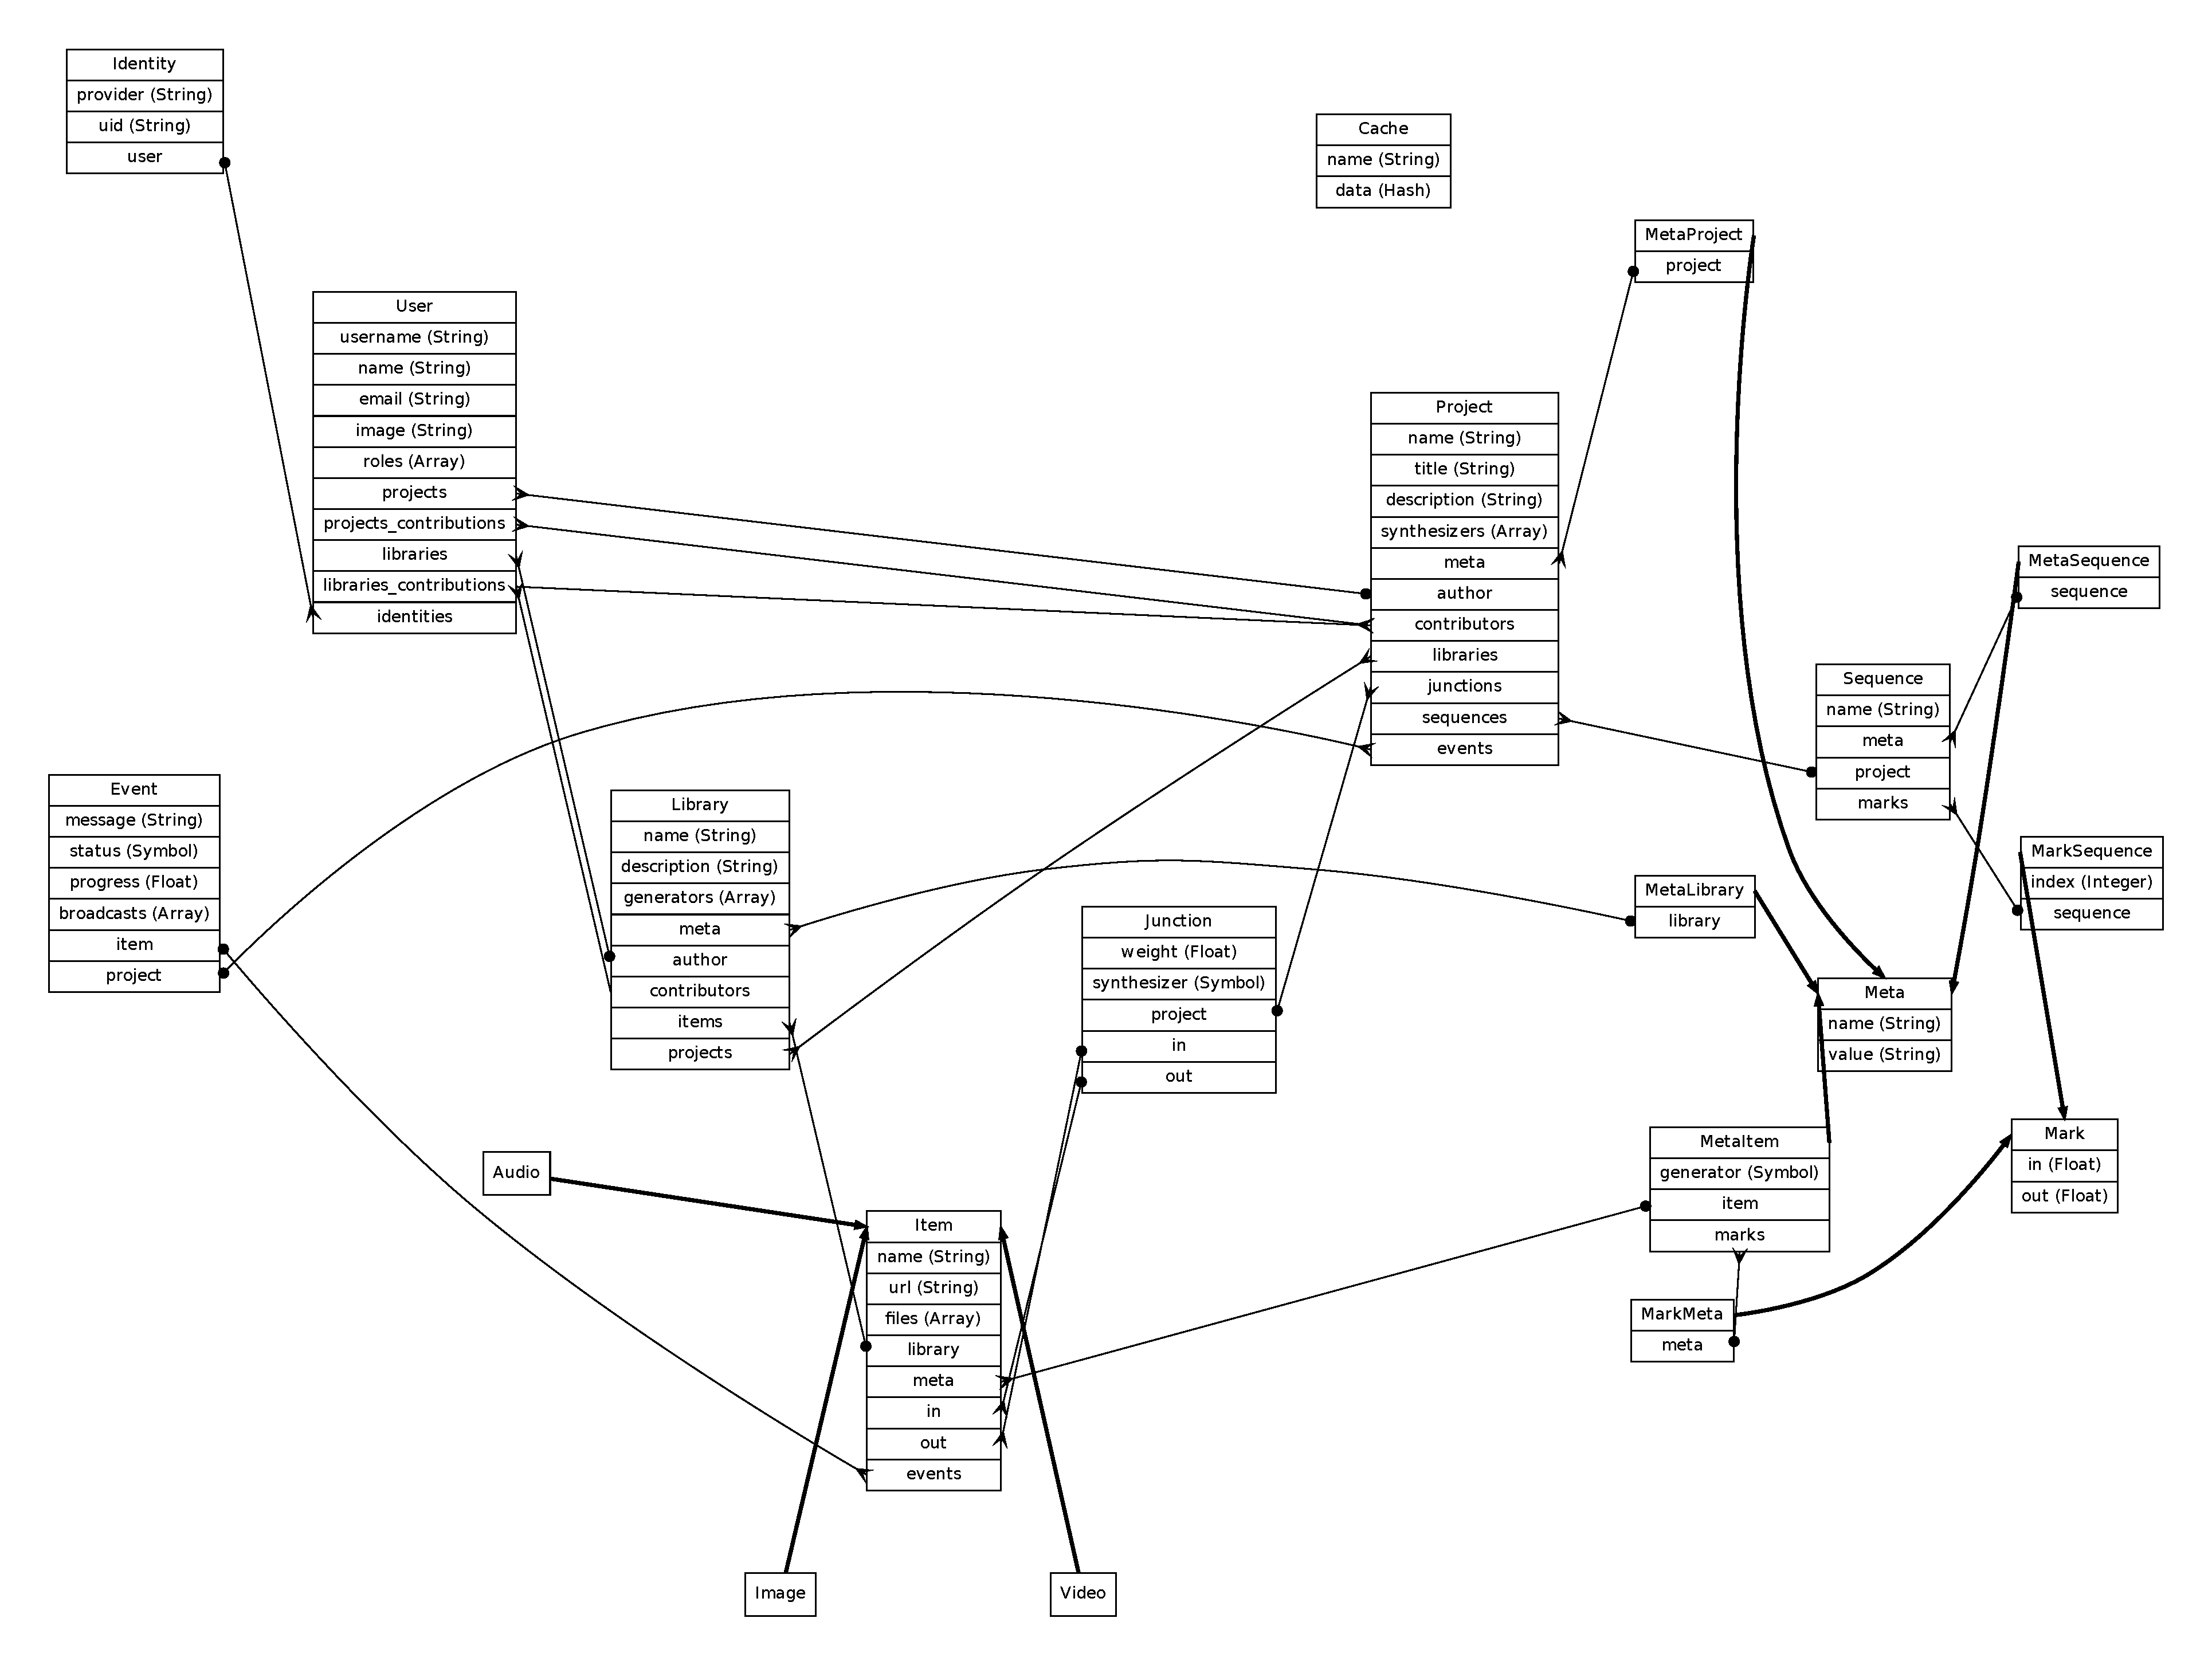
\includegraphics[width=1\textwidth]{./obrazova_priloha/domain_full.pdf}
\caption{Doménový model celého projektu Narra}
\end{figure}

\par User reprezentuje přihlášeného uživatele, který chce používat aplikaci. Každý uživatel může mít vazbu na projekt a knihovnu. Entita Item obsahuje informace o jménech souboru, url videa a vlastních stažených souborů. Dále obsahuje vazby na knihovnu ve které je uložen sám Item. Itemy se podle definice v modelu nemohou vyskytovat samostatně, musí být organizovány v knihovnách. V případě mého projektu nebudu vytvářet Item ale jeho potomka Video. 
\par Další vazba je na entity MetaItem, které reprezentují generátor pro metadata. MetaItem je třídní potomek Meta, který přebírá atributy rodiče, jež jsou povinné. Při ukládání položek v Meta musí být vyplněno Meta.name i Meta.value.

\begin{figure}[H]
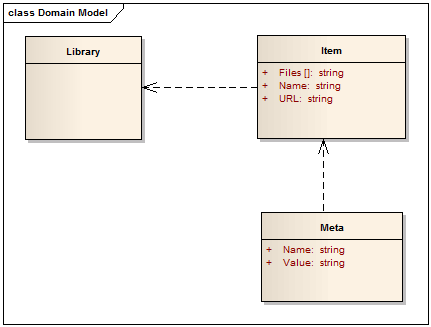
\includegraphics[width=1\textwidth]{./obrazova_priloha/domain_my.png}
\caption{Doménový model mé části Narry}
\end{figure}
\par Moje část aplikace se týká především entit Video, MetaItem a Library. Entita Library reprezentuje celou knihovnu videí, se kterou se bude lokálně pracovat. Video (potomek Item) je entita, které budu při vytváření asistovat poskytnutím URL při zadávání. Po zadání budu muset zpracovat obsah odkazu a vrátit metadata a cestu ke stažení videa. Jméno pro konkrétní prvek je reprezentováno řetězcem a url je také řetězec. Pro jednoduché volání budu mít vytvořenou třídu Connector, potomka Narra::SPI, která bude provádět inicializace, validaci, popis metadaty a stažení videa a případných titulků.
\par Zpracování videa probíhá vytvořením nového prvku (Item) v knihovně. Pro zpracování se použije POST požadavek s parametry v1/items/new (author, admin). Po zpracování dostaneme strukturu nově vytvořeného prvku (Item).
\par Příklad POST požadavku\cite{narra_en}:
\begin{verbatim} 
POST v1/items/new
url: "http://example.org/00329O-051.mov"
library: "552a328961633276b1000000" 
author: "Camera Guy"
metadata: {"description": "Some interesting description"}
\end{verbatim}
\hfill
\par Příklad odpovědi:
\begin{verbatim}
{"status":"OK","item":{
  "id":"552a338961633277b1000000",
  "name":"00329O-051",
  "url":"http://example.org/00329O-051.mov",
  "type":"video",
  "prepared":false,
  "library":{"id":"552a...b1000000","name":"Example Library"},
  "metadata":[
   {"name":"type","value":"video","generator":"source"},
   {"name":"name","value":"00329O-051","generator":"source"},
   {"name":"url","value":"url","generator":"source"},
   {"name":"library","value":"test","generator":"source"},
   {"name":"author","value":"testovaci","generator":"source"},
   {"name":"description","value":"test","generator":"bob"}
  ]
}}
\end{verbatim}
\par V odpovědi jsem musel zkrátit identifikátor knihovny, aby se mi vešel výraz na stránku. Ze stejného důvodu jsem byl nucen zkrátit hodnotu url. Zde je možné nastavit zda bude projekt veřejný. V takovém případě je možné dostat přístup pouze pro čtení za předpokladu, že je knihovna součástí projektu. Pro vyšší práva je nutností být contributor(spolupracovník) daného projektu. Získání výpisu přístupných knihoven se provádí GET požadavkem na zdroj/adresu v1/libraries(author/admin).